\documentclass[conference]{IEEEtran}
\IEEEoverridecommandlockouts
\usepackage{cite}
\usepackage{amsmath,amssymb,amsfonts}
\usepackage{graphicx}
\usepackage{textcomp}
\usepackage{xcolor}
\usepackage{siunitx}
\usepackage{booktabs}
\sisetup{detect-all}
\DeclareSIUnit\ohm{\ensuremath{\Omega}}
% generated by gpdk090_spectre/post/analyze.py from GPDK090 Spectre CSVs - do not edit
\newcommand{\AiPfHeavy}{1.38}
\newcommand{\BaseBw}{24.20}
\newcommand{\BaseFug}{--}
\newcommand{\BaseFul}{--}
\newcommand{\BaseGbw}{2.57}
\newcommand{\BaseI}{1.22}
\newcommand{\BaseInFive}{25.1}
\newcommand{\BaseInOne}{26.7}
\newcommand{\BaseInTen}{20.6}
\newcommand{\BaseIrms}{4.33}
\newcommand{\BaseIrmsTen}{2.47}
\newcommand{\BaseMoneGds}{2.64}
\newcommand{\BaseMoneI}{0.12}
\newcommand{\BaseP}{1.22}
\newcommand{\BasePMg}{--}
\newcommand{\BasePMl}{--}
\newcommand{\BasePk}{8.87}
\newcommand{\BasePvtBwHi}{35.2}
\newcommand{\BasePvtBwLo}{23.7}
\newcommand{\BasePvtIhi}{2.25}
\newcommand{\BasePvtIlo}{0.53}
\newcommand{\BasePvtNpk}{45}
\newcommand{\BasePvtNsat}{0}
\newcommand{\BasePvtPkHi}{20.6}
\newcommand{\BasePvtTrBwHi}{35.2}
\newcommand{\BasePvtTrBwLo}{23.7}
\newcommand{\BasePvtTrPkHi}{20.63}
\newcommand{\BasePvtZtHi}{46.6}
\newcommand{\BasePvtZtLo}{35.8}
\newcommand{\BaseTg}{-3.8}
\newcommand{\BaseTl}{-3.8}
\newcommand{\BaseZt}{40.5}
\newcommand{\BaseZtOhm}{106}
\newcommand{\BoneBw}{5.92}
\newcommand{\BoneFug}{1.00}
\newcommand{\BoneFul}{--}
\newcommand{\BoneGbw}{2.95}
\newcommand{\BoneI}{0.09}
\newcommand{\BoneInFive}{10.9}
\newcommand{\BoneInOne}{21.8}
\newcommand{\BoneInTen}{5.6}
\newcommand{\BoneIrms}{1.31}
\newcommand{\BoneIrmsTen}{1.37}
\newcommand{\BoneLf}{5.8}
\newcommand{\BoneMcBw}{6.85}
\newcommand{\BoneMcBwMin}{4.89}
\newcommand{\BoneMcBwSd}{2.49}
\newcommand{\BoneMcIsd}{4}
\newcommand{\BoneMcN}{200}
\newcommand{\BoneMcPkMax}{0.78}
\newcommand{\BoneMcPkN}{0}
\newcommand{\BoneMcTrBw}{6.85}
\newcommand{\BoneMcTrBwSd}{2.49}
\newcommand{\BoneMcTrPkMax}{0.78}
\newcommand{\BoneMcTrYield}{100.0}
\newcommand{\BoneMcYield}{100.0}
\newcommand{\BoneMcZt}{53.6}
\newcommand{\BoneMcZtSd}{0.93}
\newcommand{\BoneP}{0.09}
\newcommand{\BonePMg}{125}
\newcommand{\BonePMl}{--}
\newcommand{\BonePk}{0.49}
\newcommand{\BonePvtBwHi}{15.1}
\newcommand{\BonePvtBwLo}{0.4}
\newcommand{\BonePvtIhi}{0.27}
\newcommand{\BonePvtIlo}{0.01}
\newcommand{\BonePvtNpk}{10}
\newcommand{\BonePvtNsat}{0}
\newcommand{\BonePvtPkHi}{4.7}
\newcommand{\BonePvtTrBwHi}{15.1}
\newcommand{\BonePvtTrBwLo}{0.4}
\newcommand{\BonePvtTrPkHi}{4.74}
\newcommand{\BonePvtZtHi}{72.5}
\newcommand{\BonePvtZtLo}{38.0}
\newcommand{\BoneTg}{2.4}
\newcommand{\BoneTl}{-27.7}
\newcommand{\BoneZt}{53.9}
\newcommand{\BoneZtOhm}{498}
\newcommand{\BtwoBw}{5.10}
\newcommand{\BtwoFug}{--}
\newcommand{\BtwoFul}{--}
\newcommand{\BtwoGbw}{2.50}
\newcommand{\BtwoI}{0.92}
\newcommand{\BtwoInFive}{16.8}
\newcommand{\BtwoInOne}{42.9}
\newcommand{\BtwoInTen}{6.0}
\newcommand{\BtwoIrms}{2.31}
\newcommand{\BtwoIrmsTen}{2.44}
\newcommand{\BtwoLf}{3.6}
\newcommand{\BtwoP}{0.92}
\newcommand{\BtwoPMg}{--}
\newcommand{\BtwoPMl}{--}
\newcommand{\BtwoPk}{0.76}
\newcommand{\BtwoPvtBwHi}{25.2}
\newcommand{\BtwoPvtBwLo}{2.2}
\newcommand{\BtwoPvtIhi}{1.91}
\newcommand{\BtwoPvtIlo}{0.35}
\newcommand{\BtwoPvtNpk}{25}
\newcommand{\BtwoPvtNsat}{3}
\newcommand{\BtwoPvtPkHi}{15.0}
\newcommand{\BtwoPvtTrBwHi}{25.2}
\newcommand{\BtwoPvtTrBwLo}{2.2}
\newcommand{\BtwoPvtTrPkHi}{15.00}
\newcommand{\BtwoPvtZtHi}{59.2}
\newcommand{\BtwoPvtZtLo}{38.0}
\newcommand{\BtwoTg}{-7.8}
\newcommand{\BtwoTl}{-27.5}
\newcommand{\BtwoZt}{53.8}
\newcommand{\BtwoZtOhm}{491}
\newcommand{\ClCross}{132}
\newcommand{\DcBw}{7.86}
\newcommand{\DcBwHund}{3.81}
\newcommand{\DcCornerLim}{75}
\newcommand{\DcFloMax}{2.00}
\newcommand{\DcFuMax}{1.93}
\newcommand{\DcIadd}{86}
\newcommand{\DcInFive}{16.7}
\newcommand{\DcLim}{300}
\newcommand{\DcNoGainLim}{50}
\newcommand{\DcNoLim}{50}
\newcommand{\DcNoisePct}{4}
\newcommand{\DcPk}{0.35}
\newcommand{\DcPkMax}{1.44}
\newcommand{\DcPmMin}{78}
\newcommand{\DcZt}{53.55}
\newcommand{\DecAiOneFifty}{4.04}
\newcommand{\DecAiThirty}{7.76}
\newcommand{\DecAiThreeHundred}{2.32}
\newcommand{\DecAintOneFifty}{4.24}
\newcommand{\DecAintThirty}{8.46}
\newcommand{\DecAintThreeHundred}{2.27}
\newcommand{\DecPfOneFifty}{3.81}
\newcommand{\DecPfThirty}{9.66}
\newcommand{\DecPfThreeHundred}{1.68}
\newcommand{\DecPfcaOneFifty}{2.24}
\newcommand{\DecPfcaThirty}{5.79}
\newcommand{\DecPfcaThreeHundred}{1.32}
\newcommand{\EyeBaseBTeA}{12}
\newcommand{\EyeBaseBTeH}{79}
\newcommand{\EyeBaseBTeV}{89}
\newcommand{\EyeBaseBTwA}{12}
\newcommand{\EyeBaseBTwH}{83}
\newcommand{\EyeBaseBTwV}{80}
\newcommand{\EyeBoneBTeA}{51}
\newcommand{\EyeBoneBTeH}{79}
\newcommand{\EyeBoneBTeV}{84}
\newcommand{\EyeBoneBTwA}{47}
\newcommand{\EyeBoneBTwH}{92}
\newcommand{\EyeBoneBTwV}{81}
\newcommand{\EyeBtwoBTeA}{52}
\newcommand{\EyeBtwoBTeH}{79}
\newcommand{\EyeBtwoBTeV}{90}
\newcommand{\EyeBtwoBTwA}{47}
\newcommand{\EyeBtwoBTwH}{75}
\newcommand{\EyeBtwoBTwV}{77}
\newcommand{\EyeFoneBTeA}{48}
\newcommand{\EyeFoneBTeH}{83}
\newcommand{\EyeFoneBTeV}{89}
\newcommand{\EyeFoneBTwA}{51}
\newcommand{\EyeFoneBTwH}{88}
\newcommand{\EyeFoneBTwV}{78}
\newcommand{\EyeFtwoBTeA}{49}
\newcommand{\EyeFtwoBTeH}{79}
\newcommand{\EyeFtwoBTeV}{92}
\newcommand{\EyeFtwoBTwA}{52}
\newcommand{\EyeFtwoBTwH}{88}
\newcommand{\EyeFtwoBTwV}{79}
\newcommand{\EyePoneBTeA}{51}
\newcommand{\EyePoneBTeH}{88}
\newcommand{\EyePoneBTeV}{84}
\newcommand{\EyePoneBTwA}{47}
\newcommand{\EyePoneBTwH}{88}
\newcommand{\EyePoneBTwV}{90}
\newcommand{\EyePoneDUTeA}{58}
\newcommand{\EyePoneDUTeH}{92}
\newcommand{\EyePoneDUTeV}{85}
\newcommand{\EyePoneDUTwA}{56}
\newcommand{\EyePoneDUTwH}{92}
\newcommand{\EyePoneDUTwV}{90}
\newcommand{\EyePoneUTeA}{59}
\newcommand{\EyePoneUTeH}{92}
\newcommand{\EyePoneUTeV}{87}
\newcommand{\EyePoneUTwA}{57}
\newcommand{\EyePoneUTwH}{96}
\newcommand{\EyePoneUTwV}{89}
\newcommand{\EyePtwoBTeA}{52}
\newcommand{\EyePtwoBTeH}{83}
\newcommand{\EyePtwoBTeV}{81}
\newcommand{\EyePtwoBTwA}{47}
\newcommand{\EyePtwoBTwH}{79}
\newcommand{\EyePtwoBTwV}{88}
\newcommand{\EyePtwoDUTeA}{60}
\newcommand{\EyePtwoDUTeH}{88}
\newcommand{\EyePtwoDUTeV}{80}
\newcommand{\EyePtwoDUTwA}{56}
\newcommand{\EyePtwoDUTwH}{88}
\newcommand{\EyePtwoDUTwV}{86}
\newcommand{\EyePtwoUTeA}{61}
\newcommand{\EyePtwoUTeH}{88}
\newcommand{\EyePtwoUTeV}{83}
\newcommand{\EyePtwoUTwA}{58}
\newcommand{\EyePtwoUTwH}{88}
\newcommand{\EyePtwoUTwV}{87}
\newcommand{\FoneBw}{9.66}
\newcommand{\FoneFug}{3.75}
\newcommand{\FoneFul}{7.48}
\newcommand{\FoneGbw}{4.75}
\newcommand{\FoneI}{0.97}
\newcommand{\FoneInFive}{14.7}
\newcommand{\FoneInOne}{16.2}
\newcommand{\FoneInTen}{19.8}
\newcommand{\FoneIrms}{1.60}
\newcommand{\FoneIrmsTen}{1.64}
\newcommand{\FoneMcBw}{9.58}
\newcommand{\FoneMcBwMin}{8.51}
\newcommand{\FoneMcBwSd}{0.32}
\newcommand{\FoneMcIsd}{34}
\newcommand{\FoneMcN}{200}
\newcommand{\FoneMcPkMax}{0.45}
\newcommand{\FoneMcPkN}{0}
\newcommand{\FoneMcTrBw}{9.58}
\newcommand{\FoneMcTrBwSd}{0.32}
\newcommand{\FoneMcTrPkMax}{0.45}
\newcommand{\FoneMcTrYield}{100.0}
\newcommand{\FoneMcYield}{100.0}
\newcommand{\FoneMcZt}{53.9}
\newcommand{\FoneMcZtSd}{0.69}
\newcommand{\FoneP}{0.97}
\newcommand{\FonePMg}{99}
\newcommand{\FonePMl}{92}
\newcommand{\FonePk}{0.07}
\newcommand{\FonePvtBwHi}{14.5}
\newcommand{\FonePvtBwLo}{5.2}
\newcommand{\FonePvtIhi}{1.09}
\newcommand{\FonePvtIlo}{0.75}
\newcommand{\FonePvtNpk}{0}
\newcommand{\FonePvtNsat}{35}
\newcommand{\FonePvtPkHi}{0.7}
\newcommand{\FonePvtTrBwHi}{14.5}
\newcommand{\FonePvtTrBwLo}{5.2}
\newcommand{\FonePvtTrPkHi}{0.68}
\newcommand{\FonePvtZtHi}{56.0}
\newcommand{\FonePvtZtLo}{51.4}
\newcommand{\FoneTg}{8.1}
\newcommand{\FoneTl}{-11.8}
\newcommand{\FoneZt}{53.8}
\newcommand{\FoneZtOhm}{492}
\newcommand{\FtwoBw}{9.99}
\newcommand{\FtwoFug}{4.23}
\newcommand{\FtwoFul}{7.54}
\newcommand{\FtwoGbw}{4.91}
\newcommand{\FtwoI}{0.97}
\newcommand{\FtwoInFive}{14.6}
\newcommand{\FtwoInOne}{16.0}
\newcommand{\FtwoInTen}{19.8}
\newcommand{\FtwoIrms}{1.63}
\newcommand{\FtwoIrmsTen}{1.63}
\newcommand{\FtwoMcBw}{9.89}
\newcommand{\FtwoMcBwMin}{8.48}
\newcommand{\FtwoMcBwSd}{0.41}
\newcommand{\FtwoMcIsd}{34}
\newcommand{\FtwoMcN}{200}
\newcommand{\FtwoMcPkMax}{0.96}
\newcommand{\FtwoMcPkN}{0}
\newcommand{\FtwoMcTrBw}{9.89}
\newcommand{\FtwoMcTrBwSd}{0.41}
\newcommand{\FtwoMcTrPkMax}{0.96}
\newcommand{\FtwoMcTrYield}{100.0}
\newcommand{\FtwoMcYield}{100.0}
\newcommand{\FtwoMcZt}{53.9}
\newcommand{\FtwoMcZtSd}{0.83}
\newcommand{\FtwoP}{0.97}
\newcommand{\FtwoPMg}{91}
\newcommand{\FtwoPMl}{96}
\newcommand{\FtwoPk}{0.35}
\newcommand{\FtwoPvtBwHi}{14.7}
\newcommand{\FtwoPvtBwLo}{5.4}
\newcommand{\FtwoPvtIhi}{1.08}
\newcommand{\FtwoPvtIlo}{0.74}
\newcommand{\FtwoPvtNpk}{0}
\newcommand{\FtwoPvtNsat}{31}
\newcommand{\FtwoPvtPkHi}{0.9}
\newcommand{\FtwoPvtTrBwHi}{14.7}
\newcommand{\FtwoPvtTrBwLo}{5.4}
\newcommand{\FtwoPvtTrPkHi}{0.89}
\newcommand{\FtwoPvtZtHi}{55.6}
\newcommand{\FtwoPvtZtLo}{51.8}
\newcommand{\FtwoTg}{8.9}
\newcommand{\FtwoTl}{-12.9}
\newcommand{\FtwoZt}{53.8}
\newcommand{\FtwoZtOhm}{492}
\newcommand{\GfInv}{573}
\newcommand{\Gmf}{1.45}
\newcommand{\IOne}{110}
\newcommand{\IThree}{665}
\newcommand{\Imf}{104}
\newcommand{\LdBoneClOneFifty}{1.98}
\newcommand{\LdBoneClThirty}{5.93}
\newcommand{\LdBoneClThreeHundred}{1.01}
\newcommand{\LdBoneCpdOneHundred}{3.31}
\newcommand{\LdBoneCpdThreeHundred}{1.06}
\newcommand{\LdBoneCpdTwoHundred}{1.64}
\newcommand{\LdFoneClOneFifty}{3.80}
\newcommand{\LdFoneClThirty}{9.64}
\newcommand{\LdFoneClThreeHundred}{1.68}
\newcommand{\LdFoneCpdOneHundred}{nan}
\newcommand{\LdFoneCpdThreeHundred}{nan}
\newcommand{\LdFoneCpdTwoHundred}{nan}
\newcommand{\LdPoneClOneFifty}{4.04}
\newcommand{\LdPoneClThirty}{7.75}
\newcommand{\LdPoneClThreeHundred}{2.32}
\newcommand{\LdPoneCpdOneHundred}{7.10}
\newcommand{\LdPoneCpdThreeHundred}{5.03}
\newcommand{\LdPoneCpdTwoHundred}{5.81}
\newcommand{\LdPtwoClOneFifty}{4.39}
\newcommand{\LdPtwoClThirty}{8.41}
\newcommand{\LdPtwoClThreeHundred}{2.48}
\newcommand{\LdPtwoCpdOneHundred}{7.34}
\newcommand{\LdPtwoCpdThreeHundred}{nan}
\newcommand{\LdPtwoCpdTwoHundred}{nan}
\newcommand{\Mratio}{2.54}
\newcommand{\NPvt}{45}
\newcommand{\OvMOne}{56}
\newcommand{\OvMThree}{435}
\newcommand{\OvMThreeb}{174}
\newcommand{\OvMTwo}{119}
\newcommand{\OvMf}{609}
\newcommand{\PMgAtLo}{113}
\newcommand{\PMgAtNom}{109}
\newcommand{\PctBwLoss}{20}
\newcommand{\PfBwRawOneHundred}{8.56}
\newcommand{\PfBwRawThreeHundred}{5.99}
\newcommand{\PfBwRawTwoHundred}{6.96}
\newcommand{\PfPkOneHundred}{1.6}
\newcommand{\PfPkThreeHundred}{3.2}
\newcommand{\PfPkTwoHundred}{2.9}
\newcommand{\PoneBw}{7.76}
\newcommand{\PoneFug}{1.34}
\newcommand{\PoneFugHi}{1.53}
\newcommand{\PoneFugLo}{0.26}
\newcommand{\PoneFul}{6.29}
\newcommand{\PoneGbw}{3.82}
\newcommand{\PoneI}{0.97}
\newcommand{\PoneInFive}{15.8}
\newcommand{\PoneInOne}{18.3}
\newcommand{\PoneInTen}{20.7}
\newcommand{\PoneIrms}{1.51}
\newcommand{\PoneIrmsHi}{1.51}
\newcommand{\PoneIrmsLo}{1.24}
\newcommand{\PoneIrmsTen}{1.77}
\newcommand{\PoneMcBw}{7.67}
\newcommand{\PoneMcBwMin}{6.75}
\newcommand{\PoneMcBwSd}{0.35}
\newcommand{\PoneMcIsd}{31}
\newcommand{\PoneMcN}{200}
\newcommand{\PoneMcPkMax}{1.74}
\newcommand{\PoneMcPkN}{7}
\newcommand{\PoneMcTrBw}{7.77}
\newcommand{\PoneMcTrBwSd}{0.31}
\newcommand{\PoneMcTrPkMax}{1.00}
\newcommand{\PoneMcTrYield}{100.0}
\newcommand{\PoneMcVhi}{0.34}
\newcommand{\PoneMcVlo}{0.20}
\newcommand{\PoneMcYield}{96.5}
\newcommand{\PoneMcZt}{53.9}
\newcommand{\PoneMcZtSd}{0.64}
\newcommand{\PoneP}{0.97}
\newcommand{\PonePMg}{109}
\newcommand{\PonePMgMin}{108}
\newcommand{\PonePMl}{87}
\newcommand{\PonePk}{0.07}
\newcommand{\PonePkTop}{3.5}
\newcommand{\PonePvtBwHi}{11.5}
\newcommand{\PonePvtBwLo}{2.8}
\newcommand{\PonePvtIhi}{1.09}
\newcommand{\PonePvtIlo}{0.75}
\newcommand{\PonePvtNpk}{17}
\newcommand{\PonePvtNsat}{35}
\newcommand{\PonePvtPkHi}{4.5}
\newcommand{\PonePvtSlow}{SF, 125\,\si{\celsius}, 1.1\,V}
\newcommand{\PonePvtTrBwHi}{11.5}
\newcommand{\PonePvtTrBwLo}{4.0}
\newcommand{\PonePvtTrPkHi}{1.00}
\newcommand{\PonePvtTrVhi}{0.40}
\newcommand{\PonePvtTrVlo}{0.08}
\newcommand{\PonePvtWorst}{FS, -40\,\si{\celsius}, 0.9\,V}
\newcommand{\PonePvtZtHi}{56.0}
\newcommand{\PonePvtZtLo}{51.6}
\newcommand{\PoneTg}{8.1}
\newcommand{\PoneTl}{-11.8}
\newcommand{\PoneTuneMax}{7.76}
\newcommand{\PoneTuneMin}{5.70}
\newcommand{\PoneTuneRatio}{1.36}
\newcommand{\PoneVtOk}{0.24}
\newcommand{\PoneZt}{53.8}
\newcommand{\PoneZtOhm}{492}
\newcommand{\PoneZtSpread}{0.01}
\newcommand{\PtwoBw}{8.40}
\newcommand{\PtwoFug}{1.72}
\newcommand{\PtwoFugHi}{1.88}
\newcommand{\PtwoFugLo}{0.18}
\newcommand{\PtwoFul}{6.52}
\newcommand{\PtwoGbw}{4.14}
\newcommand{\PtwoI}{0.94}
\newcommand{\PtwoInFive}{15.7}
\newcommand{\PtwoInOne}{18.2}
\newcommand{\PtwoInTen}{20.6}
\newcommand{\PtwoIrms}{1.58}
\newcommand{\PtwoIrmsHi}{1.59}
\newcommand{\PtwoIrmsLo}{1.51}
\newcommand{\PtwoIrmsTen}{1.76}
\newcommand{\PtwoMcBw}{8.36}
\newcommand{\PtwoMcBwMin}{7.56}
\newcommand{\PtwoMcBwSd}{0.26}
\newcommand{\PtwoMcIsd}{30}
\newcommand{\PtwoMcN}{200}
\newcommand{\PtwoMcPkMax}{2.46}
\newcommand{\PtwoMcPkN}{80}
\newcommand{\PtwoMcTrBw}{8.35}
\newcommand{\PtwoMcTrBwSd}{0.25}
\newcommand{\PtwoMcTrPkMax}{1.00}
\newcommand{\PtwoMcTrYield}{100.0}
\newcommand{\PtwoMcVhi}{0.28}
\newcommand{\PtwoMcVlo}{0.12}
\newcommand{\PtwoMcYield}{60.0}
\newcommand{\PtwoMcZt}{53.9}
\newcommand{\PtwoMcZtSd}{0.62}
\newcommand{\PtwoP}{0.94}
\newcommand{\PtwoPMg}{103}
\newcommand{\PtwoPMgMin}{102}
\newcommand{\PtwoPMl}{83}
\newcommand{\PtwoPk}{0.43}
\newcommand{\PtwoPkTop}{4.5}
\newcommand{\PtwoPvtBwHi}{12.7}
\newcommand{\PtwoPvtBwLo}{4.3}
\newcommand{\PtwoPvtIhi}{1.05}
\newcommand{\PtwoPvtIlo}{0.74}
\newcommand{\PtwoPvtNpk}{21}
\newcommand{\PtwoPvtNsat}{36}
\newcommand{\PtwoPvtPkHi}{5.2}
\newcommand{\PtwoPvtSlow}{SF, 125\,\si{\celsius}, 0.9\,V}
\newcommand{\PtwoPvtTrBwHi}{12.6}
\newcommand{\PtwoPvtTrBwLo}{4.9}
\newcommand{\PtwoPvtTrPkHi}{0.96}
\newcommand{\PtwoPvtTrVhi}{0.40}
\newcommand{\PtwoPvtTrVlo}{0.00}
\newcommand{\PtwoPvtWorst}{FS, -40\,\si{\celsius}, 0.9\,V}
\newcommand{\PtwoPvtZtHi}{56.2}
\newcommand{\PtwoPvtZtLo}{51.4}
\newcommand{\PtwoTg}{8.6}
\newcommand{\PtwoTl}{-12.6}
\newcommand{\PtwoTuneMax}{8.43}
\newcommand{\PtwoTuneMin}{7.95}
\newcommand{\PtwoTuneRatio}{1.06}
\newcommand{\PtwoVtOk}{0.20}
\newcommand{\PtwoZt}{53.9}
\newcommand{\PtwoZtOhm}{493}
\newcommand{\PtwoZtSpread}{0.01}
\newcommand{\QmaxD}{0.17}
\newcommand{\RatioBwFonePone}{1.24}
\newcommand{\RatioBwPoneBone}{1.31}
\newcommand{\RatioIPoneBone}{10.9}
\newcommand{\RcBwHi}{7.81}
\newcommand{\RcBwLo}{7.54}
\newcommand{\RcPkHi}{0.60}
\newcommand{\RcZtHi}{54.3}
\newcommand{\RcZtLo}{53.5}
\newcommand{\Ro}{954}
\newcommand{\Tzero}{3.50}
\newcommand{\TzeroStb}{2.54}
\newcommand{\VcrossPred}{0.214}
\newcommand{\VcrossSim}{0.236}
\newcommand{\Vin}{0.28}
\newcommand{\Vout}{0.61}
\newcommand{\VtwoCa}{22.7}
\newcommand{\VtwoDistinct}{yes}
\newcommand{\VtwoIref}{48.9}
\newcommand{\VtwoRn}{5.44}
\newcommand{\VtwoVt}{0.18}
\newcommand{\VtwoWF}{3.42}
\newcommand{\VtwoWT}{6.80}
\newcommand{\VtwoWa}{3.17}
\newcommand{\VtwoWb}{3.10}
\newcommand{\VtwoWc}{6.22}
\newcommand{\VtwoWcB}{27.21}
\newcommand{\ZaiLA}{-6.1}
\newcommand{\ZaiLB}{0.4}
\newcommand{\ZaiLC}{9.7}
\newcommand{\ZaiLD}{33.2}
\newcommand{\ZaiLpA}{-4.4}
\newcommand{\ZaiLpB}{3.4}
\newcommand{\ZaiLpC}{14.7}
\newcommand{\ZaiLpD}{43.3}
\newcommand{\ZaiR}{573}
\newcommand{\ZaiRtA}{351}
\newcommand{\ZaiRtB}{745}
\newcommand{\ZaiRtC}{1315}
\newcommand{\ZaiRtD}{2754}
\newcommand{\ZtApprox}{538}
\newcommand{\ZtErr}{9}

\makeatletter\let\tableinput\@@input\makeatother

\begin{document}

\title{Where Does Tunable Gyrator-C Feedback Help an Inductorless Current-Mirror TIA? A Gain-Matched GPDK090 Study}

% Double-blind submission: author block removed. Camera-ready block below.
\author{\IEEEauthorblockN{Anonymous Authors}\IEEEauthorblockA{\textit{Affiliation withheld for review}}}
%\author{\IEEEauthorblockN{Shreyas S, Vidhula Vanmaye, Prakruthi V Raj, Narsepalli Sreekar, and Shyleshree}
%\IEEEauthorblockA{\textit{Dept. of Electronics and Communication Engineering, R V College of Engineering}, Bengaluru, India}}

\maketitle

\begin{abstract}
A 2020 current-mirror transimpedance amplifier (TIA) closes its loop with a \SI{2.4}{nH} spiral. Simulated as drawn with the Cadence GPDK090 generic kit, its common-gate device carries \BaseMoneI\,nA, the gain is \BaseZt\,dB$\Omega$ and the response peaks by \BasePk\,dB. We bias the input as a flipped voltage follower and replace the spiral with a source follower whose gate is fed from the output through a triode PMOS, so one voltage $V_{tune}$ moves the feedback zero. With a \SI{50}{fF} photodiode, a \SI{30}{fF} load and \SI{1}{V}, Spectre gives \PoneZt\,dB$\Omega$ and \PoneBw\,GHz at \PoneI\,mA, tunable from \PoneTuneMin\ to \PoneTuneMax\,GHz with under \SI{1}{dB} of peaking. All comparisons are at equal gain. A spiral TIA re-optimised on the same kit reaches \BoneBw\,GHz at \BoneI\,mA, and an untuned source follower at the same current reaches \FoneBw\,GHz, because the gyrator network adds capacitance at the input. The tunable network wins where a fixed one cannot adapt: re-tuned, it holds peaking under \SI{1}{dB} with a \SI{300}{fF} photodiode, where the plain follower peaks by \PfPkThreeHundred\,dB; it overtakes the plain follower above about \ClCross\,fF of load; and it trims all \NPvt\ corner points and 200 mismatch samples to under \SI{1}{dB}. A version re-sized for bandwidth reaches \PtwoBw\,GHz but keeps only a \PtwoTuneRatio:1 tuning range. A DC-cancellation loop extends the photocurrent range to \DcLim\,\si{\micro A}. All results are schematic-level simulations.
\end{abstract}

\begin{IEEEkeywords}
transimpedance amplifier, active inductor, gyrator-C, current mirror, flipped voltage follower, bandwidth tuning, GPDK090
\end{IEEEkeywords}

\section{Introduction}
The TIA sets most of the noise and much of the bandwidth of an optical receiver \cite{razavi,sackinger}. Current-mirror TIAs operate from \SI{1}{V} because the signal remains a current until the output node, and several have been reported in 45 to 90\,nm CMOS \cite{zohoori,hassan,issa,alyas,shaaban}. Bandwidth is usually extended with spiral inductors \cite{mohanbw}, which occupy far more area than the transistors and are fixed once fabricated. Active inductors trade noise and power for area and tunability \cite{yuan,razaviai}; they have been used as loads \cite{zohoori}, as shunt peaking \cite{shaaban,kumar} and as local feedback \cite{alberwari,alyas} in TIAs, and inductorless active feedback has extended the bandwidth of regulated-cascode TIAs \cite{chen16}. Measured CMOS TIAs with a bandwidth control voltage exist \cite{hwang,chien}. The active-inductor TIAs closest to this work \cite{alberwari,alyas} use PMOS active inductors as local feedback around single stages and are not tunable; here the gyrator network replaces the global output-to-input spiral of a current-mirror TIA, and its triode resistor is the tuning element. We do not claim the network itself as new. What we add is a measurement, at equal gain, of what it costs and what it buys.

Alsheikhjader \cite{baseline} reported a 90\,nm, \SI{1}{V} current-mirror TIA with a \SI{2.4}{nH} spiral from output to input and a flat \SIrange{5}{15}{GHz} response at \SI{43.9}{dB\ohm}, without power, photodiode capacitance or device model. Replacing that spiral with a tunable source-follower network is easy to propose; showing that it helps is harder, because an untuned source follower already provides output-to-input feedback and a well-biased spiral TIA is efficient. This paper therefore compares four feedback options at equal transimpedance with the GPDK090 v4.6 generic process design kit (not a foundry process) and Spectre 12.1. Its contributions are:
\begin{enumerate}
\item A check of the 2020 circuit as drawn, showing that its input device is in triode and that its published response does not follow from the schematic (Section~\ref{sec:base}).
\item A gain-matched comparison of spiral, plain-follower and tunable gyrator-C feedback that separates the cost of each element of the gyrator network and identifies where the tunable network wins: large photodiode capacitance, heavy load, and corner and mismatch trimming (Sections~\ref{sec:cmp}--\ref{sec:rob}).
\item A verified small-signal account of the network: it is resistive at $1/g_f$, becomes inductive only when $R_t>1/g_f$, and over the useful tuning range acts as a movable zero rather than a resonator (Section~\ref{sec:prop}).
\end{enumerate}
All numbers in this paper are from schematic-level Spectre runs, with ideal resistors and capacitors; there is no layout, extraction or silicon.

\begin{figure}[t]
\centering
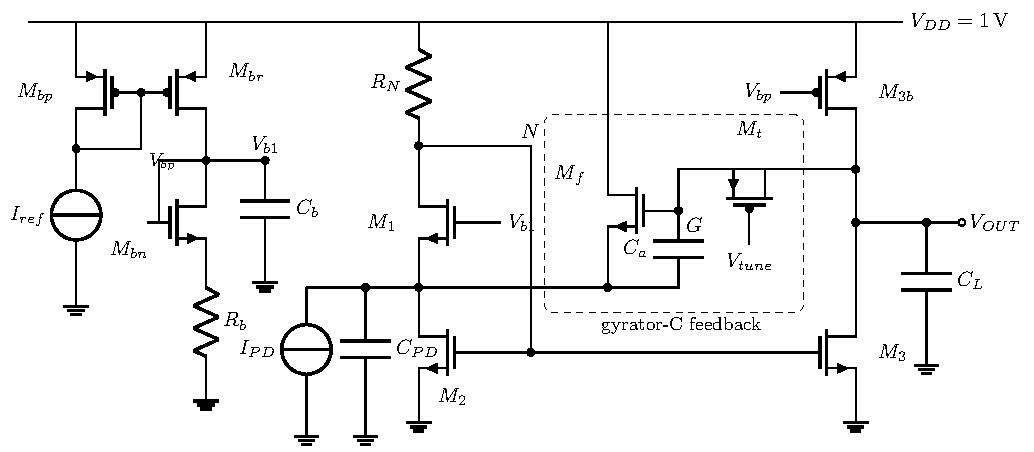
\includegraphics[width=\linewidth]{figures/schem_proposed}\\[2pt]
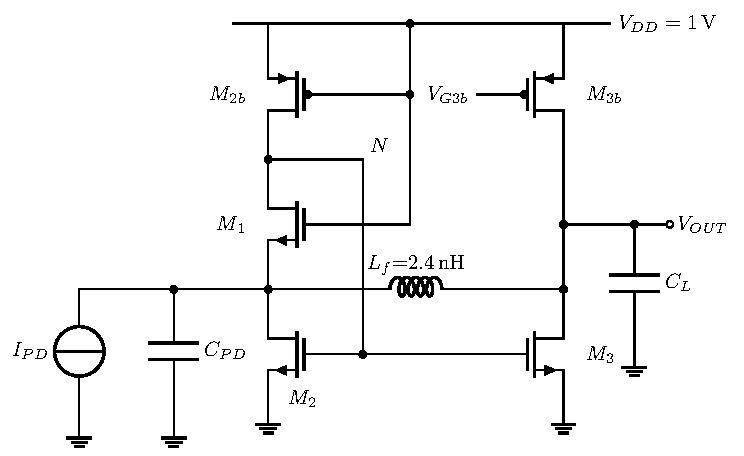
\includegraphics[width=0.66\linewidth]{figures/schem_baseline}
\caption{Top: proposed TIA with its bias generator. Plain-follower feedback (F1) ties the gate of $M_f$ to $V_{OUT}$ and removes $M_t$ and $C_a$. Bottom: the 2020 TIA \cite{baseline}; the re-optimised baselines B1 and B2 give $M_{2b}$ its own gate bias and add a series loss to $L_f$.}
\label{fig:schem}
\end{figure}

\section{The 2020 Circuit and a Fair Reference}\label{sec:base}
In the published schematic (Fig.~\ref{fig:schem}, bottom) the gates of $M_1$ and $M_{2b}$ are tied to $V_{DD}$. $M_{2b}$ then has zero gate-source voltage, so $M_1$ carries \BaseMoneI\,nA and acts as a \BaseMoneGds\,mS switch between node $N$ and the input. With $C_{PD}=\SI{50}{fF}$ and $C_L=\SI{30}{fF}$, both assumed here and throughout, the circuit gives \BaseZt\,dB$\Omega$ with \BasePk\,dB of peaking near \SI{18}{GHz} (Fig.~\ref{fig:ac}a): as $\omega L_f$ grows the feedback falls away and the gain rises until node capacitances take over. A fit of the topology to points digitised from \cite{baseline}, done earlier with a predictive model, matched the published curve only when $L_f$ was reduced below about \SI{30}{pH}. We conclude that the published response does not come from the circuit as drawn, and we do not compare against it.

The reference is instead the same topology re-optimised on GPDK090 for maximum bandwidth with $M_{2b}$ given its own gate bias, $L_f$ from 0.2 to \SI{6}{nH} with up to \SI{60}{\ohm} of series loss, widths from 0.2 to \SI{15}{\micro m}, at most \SI{1}{dB} of peaking and \SI{1.2}{mW}, every device in saturation, and at least the proposed circuit's \PoneZt\,dB$\Omega$ (B1). A second run forces at least \SI{0.9}{mA} (B2) to show what the spiral topology does with the proposed circuit's current. Both used differential evolution followed by a local search, with the same constraints and the same Spectre test bench as the proposed circuit.

\section{Proposed Circuit}\label{sec:prop}
\subsection{Topology and bias}
The proposed TIA (Fig.~\ref{fig:schem}, top) changes three things. $M_{2b}$ becomes $R_N=\SI{5}{k\ohm}$ and $M_1$ is biased from $V_{b1}$, so $M_1$ carries \IOne\,\si{\micro A} in saturation and $M_1$--$M_2$ form a flipped voltage follower \cite{fvf} that lowers the input resistance as a regulated cascode does \cite{park}. $M_{3b}$ and $V_{b1}$ come from a \SI{50}{\micro A} reference through $M_{bp}$, $M_{br}$ and a diode-connected replica $M_{bn}$ with $R_b$. The spiral is replaced by the source follower $M_f$, whose gate $G$ is fed from $V_{OUT}$ through the triode PMOS $M_t$ (gate $V_{tune}$), with $C_a$ between $G$ and the input. $M_t$ carries no DC current, so $V_{tune}$ does not move the operating point; the input sits at \Vin\,V and the output at \Vout\,V. Sizes are in Table~\ref{tab:sizes}. The smallest saturation margin, $V_{DS}-V_{DSAT}$, is \OvMOne\,mV, in $M_1$.

\begin{table}[t]
\caption{Device sizes, $W/L$ in \si{\micro m} (v1). $R_N=\SI{5}{k\ohm}$, $R_b=\SI{4.2}{k\ohm}$, $C_a=\SI{30}{fF}$, $C_b=\SI{2}{pF}$, $I_{ref}=\SI{50}{\micro A}$}
\label{tab:sizes}
\centering\footnotesize\setlength{\tabcolsep}{4pt}
\begin{tabular}{llll}
\toprule
$M_1$ & 4.5/0.1 & $M_f$ & 3.5/0.1 \\
$M_2$ & 3.5/0.1 & $M_t$ (PMOS) & 12/0.1 \\
$M_3$ & 7/0.1 & $M_{bp}$, $M_{br}$ (PMOS) & 2/0.18 \\
$M_{3b}$ (PMOS) & 28/0.18 & $M_{bn}$ & 0.4/0.1 \\
\bottomrule
\end{tabular}
\end{table}

\subsection{The gyrator-C network}
With the output at AC ground, $M_f$ and its gate network present to the input
\begin{equation}
Z_{AI}=\frac{1+sR_tC_g}{g_f+sC_g},\qquad L_{eq}=\frac{C_g}{g_f}\left(R_t-\frac{1}{g_f}\right),
\label{eq:zai}
\end{equation}
where $g_f=g_{mf}+g_{mbf}+g_{dsf}$, $C_g=C_a+C_{gs,f}$ and $R_t$ is the channel resistance of $M_t$ \cite{yuan}. From the operating point, $1/g_f=\GfInv\,\Omega$; Spectre gives a low-frequency $|Z_{AI}|$ of \ZaiR\,$\Omega$ (Fig.~\ref{fig:zai}). Equation~(\ref{eq:zai}) predicts that the element turns inductive when $R_t$ exceeds $1/g_f$, at $V_{tune}=\VcrossPred$\,V; the simulated sign change is at \VcrossSim\,V. At $V_{tune}=0.28$ and \SI{0.32}{V} ($R_t=\ZaiRtC$ and \ZaiRtD\,$\Omega$) the simulated $L_{eq}$ at \SI{100}{MHz} is \ZaiLC\ and \ZaiLD\,nH against \ZaiLpC\ and \ZaiLpD\,nH predicted; the formula ignores $C_{gd}$ and junction capacitance and overestimates. The peak quality factor is only \QmaxD. Over the range used for flat responses, $V_{tune}\le\PoneVtOk$\,V, the network is not inductive at all: it is a resistive-capacitive branch whose zero $1/(R_tC_g)$ moves with $V_{tune}$.

\begin{figure}[t]
\centering
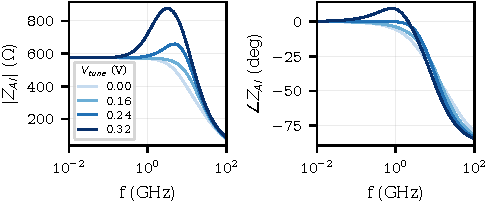
\includegraphics[width=\linewidth]{figures/g_zai}
\caption{Impedance of the gyrator-C network seen from the input, output held at its DC value (GPDK090, NN, \SI{35}{\celsius}).}
\label{fig:zai}
\end{figure}

\subsection{Transimpedance}
Let $m=g_{m3}/g_{m2}$ and $R_o=1/(g_{ds3}+g_{ds3b})$. Closing the loop through $M_f$ gives
\begin{equation}
Z_T(s)\approx-\frac{mR_o(1+sR_tC_g)}{(1+sR_oC_o)(1+sR_tC_g)+m\,g_{mf}R_o}\,H_{in}(s),
\label{eq:zt}
\end{equation}
with $H_{in}$ the second-order response of the input stage. At DC, $Z_T=-mR_o/(1+T_0)$ with $T_0=mg_{mf}R_o$. From the operating point $m=\Mratio$, $R_o=\Ro\,\Omega$ and $T_0=\Tzero$, so $|Z_T|=\ZtApprox\,\Omega$ against \PoneZtOhm\,$\Omega$ from Spectre (\ZtErr\,\% high). Spectre's loop-gain analysis at the follower's source gives $T_0=\TzeroStb$; the difference is the input-stage loading that (\ref{eq:zt}) folds into $H_{in}$. The zero at $1/(R_tC_g)$ cancels part of the output pole: a small $R_t$ removes the feedback early and the response droops, a larger one flattens it, and a still larger one turns the network inductive and the response peaks.

\section{Gain-Matched Comparison}\label{sec:cmp}
Table~\ref{tab:nom} and Fig.~\ref{fig:ac} give the nominal results (NN, \SI{35}{\celsius}, \SI{1}{V}). Noise is input-referred; $i_{n,rms}$ is integrated from \SI{10}{MHz} to each circuit's bandwidth. Integrated to a common \SI{10}{GHz} it is \PoneIrmsTen\,\si{\micro A} for v1, \FoneIrmsTen\ for F1 and \BoneIrmsTen\ for B1. For a bit-error rate of $10^{-12}$ ($Q=7$), v1's \PoneIrms\,\si{\micro A} corresponds to a minimum input of about \SI{21}{\micro A} peak to peak, ignoring the noise of later stages.

\begin{table}[t]
\caption{Nominal comparison, GPDK090, $C_{PD}=\SI{50}{fF}$, $C_L=\SI{30}{fF}$}
\label{tab:nom}
\centering\footnotesize\setlength{\tabcolsep}{2.2pt}
\begin{tabular}{lccccccc}
\toprule
Circuit & Gain & Peak & BW & $I_{DD}$ & $i_n$@5G & $i_{n,rms}$ & Feedback \\
 & dB$\Omega$ & dB & GHz & mA & pA/$\sqrt{\rm Hz}$ & \si{\micro A} & \\
\midrule
\tableinput table_nominal.tex
\bottomrule
\end{tabular}
\end{table}

\begin{figure*}[t]
\centering
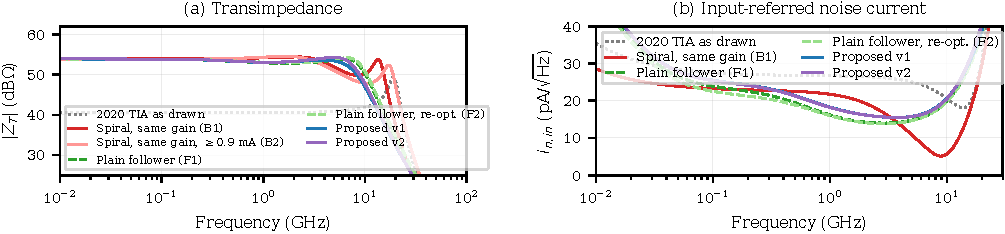
\includegraphics[width=\textwidth]{figures/g_ac_noise}
\caption{(a) Transimpedance and (b) input-referred noise current of every circuit, GPDK090, NN, \SI{35}{\celsius}, \SI{1}{V}.}
\label{fig:ac}
\end{figure*}

\emph{Against the spiral.} B1 reaches \BoneBw\,GHz at \BoneI\,mA and has the lowest noise above about \SI{4}{GHz} and the lowest integrated noise. The proposed circuit reaches \PoneBw\,GHz, \RatioBwPoneBone\ times as much, for \RatioIPoneBone\ times the current. B1's gain is $1/(g_{m2}+g_{m3})$, so matching \PoneZt\,dB$\Omega$ forces small mirror devices; the optimiser drove $M_1$ and $M_2$ to the \SI{0.2}{\micro m} width limit. Forced to draw at least \SI{0.9}{mA} (B2), the topology does worse, \BtwoBw\,GHz with more noise: extra current raises $g_m$, which the gain constraint does not allow. On efficiency the spiral TIA wins clearly. The proposed circuit removes a \BoneLf-nH spiral and adds a control input.

\emph{Against the plain follower.} At the same gain and current F1 reaches \FoneBw\,GHz, \PctBwLoss\,\% more than the proposed circuit, with slightly less noise. Fig.~\ref{fig:loads}(c) splits the gyrator network into its parts at the v1 sizes. Adding only $C_a$ between output and input of the plain follower cuts the bandwidth to \DecPfcaThirty\,GHz; adding only $M_t$ with $C_{gs,f}$ gives \DecAintThirty\,GHz; the full network gives \DecAiThirty\,GHz. At \SI{30}{fF} the bandwidth is set by the input node, and every capacitance the network adds there costs bandwidth. The inductive zero only pays when the output pole dominates.

\section{Load, Photodiode and Tuning}\label{sec:load}
Fig.~\ref{fig:tune} gives the tuning law. Between 0 and \PoneVtOk\,V the bandwidth moves from \PoneTuneMin\ to \PoneTuneMax\,GHz with the gain constant to \PoneZtSpread\,dB and peaking below \SI{0.1}{dB}; above that the network turns inductive and peaking grows to \PonePkTop\,dB. The integrated input noise falls from \PoneIrmsHi\ to \PoneIrmsLo\,\si{\micro A} at the lower settings, which suits lower data rates. Loop gains were taken with Spectre's stability analysis, with probes in series with the follower's source (global loop) and with the gate of $M_2$ (local flipped-voltage-follower loop). The global loop has \PoneTg\,dB of low-frequency gain, crosses unity at \PoneFug\,GHz and keeps at least \PonePMgMin\si{\degree} of phase margin over the whole tuning range (Table~\ref{tab:tune}); the local loop crosses at \PoneFul\,GHz with \PonePMl\si{\degree} (Fig.~\ref{fig:stb}). The peaking above \PoneVtOk\,V is therefore not a stability problem: it comes from the zero overshooting the output pole, not from a loss of margin.

\begin{table}[t]
\caption{Tuning law of v1 (GPDK090, NN, \SI{35}{\celsius}); $R_t$ from the operating point, $i_{n,rms}$ to the bandwidth}
\label{tab:tune}
\centering\footnotesize\setlength{\tabcolsep}{3pt}
\begin{tabular}{ccccccc}
\toprule
$V_{tune}$ & $R_t$ & BW & Peak & $i_n$@5G & $i_{n,rms}$ & PM$_g$ \\
V & $\Omega$ & GHz & dB & pA/$\sqrt{\rm Hz}$ & \si{\micro A} & deg \\
\midrule
\tableinput table_tune.tex
\bottomrule
\end{tabular}
\end{table}

\begin{figure}[t]
\centering
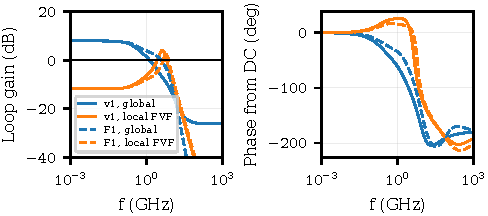
\includegraphics[width=\linewidth]{figures/g_stb}
\caption{Global and local loop gains of v1 ($V_{tune}=\SI{0.24}{V}$, solid) and F1 (dashed), GPDK090, NN, \SI{35}{\celsius}.}
\label{fig:stb}
\end{figure}

\begin{figure}[t]
\centering
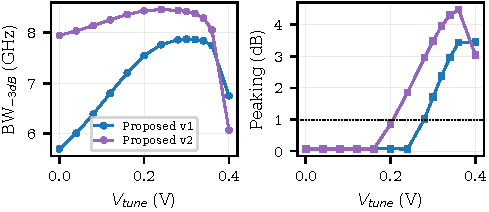
\includegraphics[width=\linewidth]{figures/g_tuning}
\caption{Bandwidth and peaking against $V_{tune}$ (GPDK090, NN, \SI{35}{\celsius}).}
\label{fig:tune}
\end{figure}

\begin{figure*}[t]
\centering
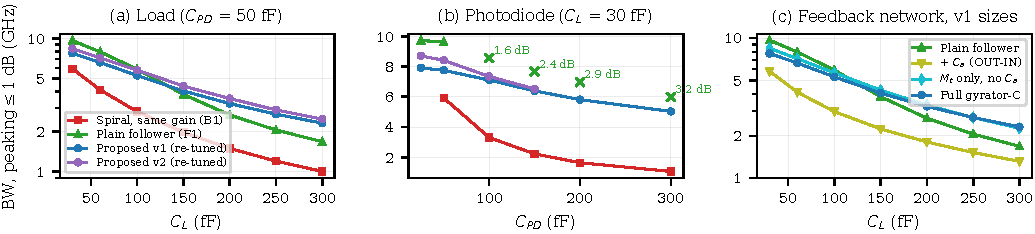
\includegraphics[width=\textwidth]{figures/g_loads}
\caption{Largest bandwidth with no more than \SI{1}{dB} of peaking. The proposed circuit is re-tuned on a \SI{20}{mV} grid at each point; B1 and F1 have no tuning input. (a) Against $C_L$. (b) Against $C_{PD}$; crosses mark F1, whose peaking exceeds \SI{1}{dB}. (c) The gyrator network taken apart at the v1 sizes.}
\label{fig:loads}
\end{figure*}

Fig.~\ref{fig:loads} and Table~\ref{tab:where} show where the tuning input matters. With a larger load (a), re-tuning moves the zero onto the output pole; the proposed circuit passes F1 above about \ClCross\,fF and gives \AiPfHeavy\ times its bandwidth at \SI{300}{fF}. With a larger photodiode (b), F1 has no means of reducing its peaking, which reaches \PfPkOneHundred\,dB at \SI{100}{fF} and \PfPkThreeHundred\,dB at \SI{300}{fF}. Lowering $V_{tune}$ keeps the proposed circuit under \SI{1}{dB}, at \LdPoneCpdOneHundred, \LdPoneCpdTwoHundred\ and \LdPoneCpdThreeHundred\,GHz for 100, 200 and \SI{300}{fF}. B1 stays flat but falls to \LdBoneCpdThreeHundred\,GHz at \SI{300}{fF}. One die can therefore serve photodiodes of different size, which a fixed network cannot.

\subsection{Re-sizing for bandwidth (v2)}
Re-optimising the same topology for bandwidth, with gain, peaking at most \SI{0.5}{dB}, current no higher than v1 and saturation as constraints, gives v2: $C_a=\VtwoCa$\,fF, $W_t=\VtwoWT$\,\si{\micro m}, $W_1=\VtwoWa$\,\si{\micro m} and $V_{tune}=\VtwoVt$\,V. It reaches \PtwoBw\,GHz at \PtwoI\,mA (Table~\ref{tab:nom}), \SI{8}{\percent} more bandwidth for \SI{4}{\percent} less current. The price is the tuning range: v2 stays under \SI{1}{dB} only from \PtwoTuneMin\ to \PtwoTuneMax\,GHz, and \PtwoMcPkN\ of 200 mismatch samples peak above \SI{1}{dB} at its nominal setting against \PoneMcPkN\ for v1. Its smaller $C_a$ moves it toward the plain follower, which is faster and less adjustable. Because the useful properties of the network all come from the tuning range, v1 is the design we recommend, and the rest of the paper uses it.

\begin{table}[t]
\caption{Where each feedback option wins (GPDK090, equal gain)}
\label{tab:where}
\centering\footnotesize\setlength{\tabcolsep}{2.4pt}
\begin{tabular}{lccc}
\toprule
 & B1 spiral & F1 follower & Proposed v1 \\
\midrule
BW, nominal (GHz) & \BoneBw & \FoneBw & \PoneBw \\
$I_{DD}$ (mA) & \BoneI & \FoneI & \PoneI \\
BW, $C_L=\SI{300}{fF}$ (GHz) & \LdBoneClThreeHundred & \LdFoneClThreeHundred & \LdPoneClThreeHundred \\
BW, $C_{PD}=\SI{300}{fF}$, $\leq$\SI{1}{dB} (GHz) & \LdBoneCpdThreeHundred & -- (\PfPkThreeHundred\,dB) & \LdPoneCpdThreeHundred \\
Worst PVT peaking (dB) & \BonePvtPkHi & \FonePvtPkHi & \PonePvtTrPkHi\ (trimmed) \\
Spiral & \BoneLf\,nH & none & none \\
Bandwidth control & no & no & \PoneTuneRatio:1 \\
\bottomrule
\end{tabular}
\end{table}

\section{Robustness}\label{sec:rob}
\subsection{Process, supply and temperature}
The \NPvt\ conditions combine the kit's NN, SS, FF, SF and FS sections with \SIlist{-40;35;125}{\celsius} and 0.9, 1.0 and \SI{1.1}{V}. With $V_{tune}$ fixed at \SI{0.24}{V}, the proposed circuit's gain stays within \PonePvtZtLo--\PonePvtZtHi\,dB$\Omega$ and its current within \PonePvtIlo--\PonePvtIhi\,mA; \PonePvtNpk\ conditions peak above \SI{1}{dB}, worst \PonePvtPkHi\,dB at \PonePvtWorst. Choosing $V_{tune}$ per condition on the same grid brings every condition under \SI{1}{dB} (Fig.~\ref{fig:pvt}a), with bandwidths from \PonePvtTrBwLo\ to \PonePvtTrBwHi\,GHz; the slowest is \PonePvtSlow, where $V_{tune}$ reaches the top of its range. F1 stays below \FonePvtPkHi\,dB without trimming, so trimming corrects a weakness the network itself introduces. B1's gate biases are fixed voltages that do not track a reference; its gain moves from \BonePvtZtLo\ to \BonePvtZtHi\,dB$\Omega$ and its peaking reaches \BonePvtPkHi\,dB, so a fair spiral design would also need a replica bias. In \PonePvtNsat\ of \NPvt\ conditions every device of the proposed circuit and of F1 stays in saturation; the exceptions are slow, hot or low-supply corners, where $M_1$'s \OvMOne\,mV margin is used up.

\begin{figure}[t]
\centering
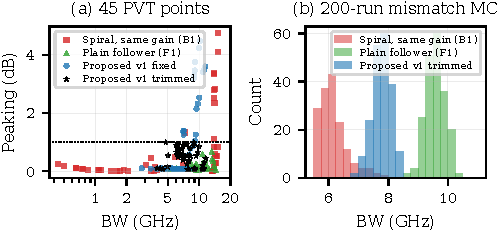
\includegraphics[width=\linewidth]{figures/g_pvt_mc}
\caption{(a) Peaking against bandwidth over \NPvt\ PVT points. (b) Bandwidth over 200 mismatch Monte Carlo samples (GPDK090 mismatch statistics, NN, \SI{35}{\celsius}).}
\label{fig:pvt}
\end{figure}

\subsection{Mismatch}
A 200-sample Monte Carlo run with the kit's mismatch statistics gives the proposed circuit $\PoneMcBw\pm\PoneMcBwSd$\,GHz and $\PoneMcZt\pm\PoneMcZtSd$\,dB$\Omega$ with $V_{tune}$ fixed, and \PoneMcPkN\ samples peak above \SI{1}{dB} (worst \PoneMcPkMax\,dB). With per-sample trimming every sample is under \SI{1}{dB}, at $\PoneMcTrBw\pm\PoneMcTrBwSd$\,GHz, using $V_{tune}$ from \PoneMcVlo\ to \PoneMcVhi\,V. B1 and F1 have \BoneMcPkN\ and \FoneMcPkN\ samples above \SI{1}{dB}. The kit provides only mismatch statistics, so global process spread is covered by the corners above, not by this run.

\subsection{Average photocurrent and DC cancellation}
Average photocurrent entering the input is drawn from $M_f$, which carries \Imf\,\si{\micro A}. Without help the gain moves by more than \SI{1}{dB} at \DcNoGainLim\,\si{\micro A}, and at \SI{100}{\micro A} the bandwidth has fallen to \DcBwHund\,GHz (Fig.~\ref{fig:dcc}a). Because $M_t$ carries no DC current, $V_{OUT}-V_{IN}$ equals $V_{GS}$ of $M_f$. A half-width replica of $M_f$ biased at half a threshold current $I_{th}$, set \SI{8}{\percent} above the dark follower current, produces $V_{OUT}-V_{GS}(I_{th})$; a PMOS-input OTA integrates its difference from $V_{IN}$ on \SI{2}{pF} and drives a sink transistor at the input (Fig.~\ref{fig:dccs}). With the loop, gain stays within \SI{1}{dB} and bandwidth within \SI{10}{\percent} of the dark values up to \DcLim\,\si{\micro A} at NN, and in every process section up to \DcCornerLim\,\si{\micro A}; in the SF section the bandwidth criterion fails first, while the gain stays within \SI{1}{dB} up to \SI{200}{\micro A}. The loop adds \DcIadd\,\si{\micro A}, \DcNoisePct\,\% of input noise at \SI{5}{GHz} and up to \DcPkMax\,dB of peaking, has at least \DcPmMin\si{\degree} of phase margin, and its low-frequency corner rises to \DcFloMax\,MHz, which limits run lengths.

\begin{figure}[t]
\centering
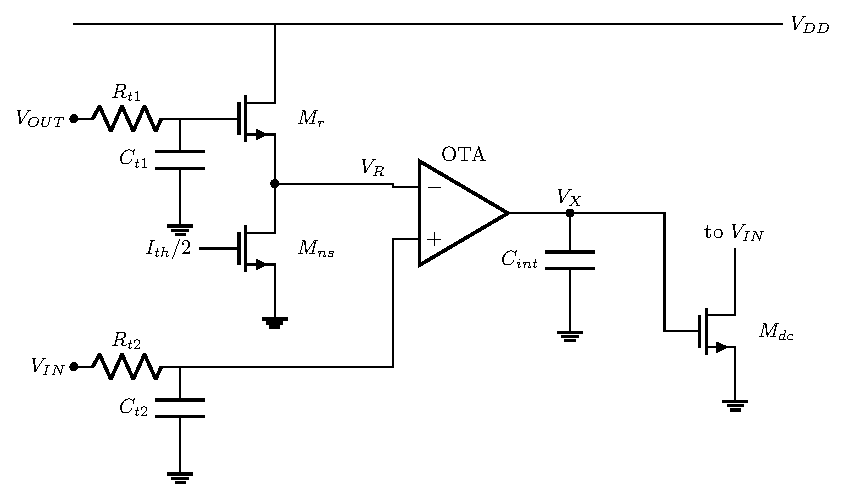
\includegraphics[width=0.85\linewidth]{figures/schem_dcc}
\caption{DC-cancellation loop. $M_r$ is half the width of $M_f$; $R_t=\SI{100}{k\ohm}$, $C_t=\SI{0.2}{pF}$, $C_{int}=\SI{2}{pF}$.}
\label{fig:dccs}
\end{figure}

\begin{figure}[t]
\centering
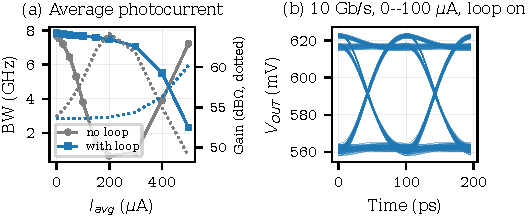
\includegraphics[width=\linewidth]{figures/g_dcc_eye}
\caption{(a) Bandwidth (solid) and gain (dotted) against average photocurrent, without and with the DC-cancellation loop. (b) Eye at \SI{10}{Gb/s}, PRBS-7, 0 to \SI{100}{\micro A}, loop on, no noise.}
\label{fig:dcc}
\end{figure}

\subsection{Eye diagrams}
For a $2^7-1$ sequence of \SI{100}{\micro A} peak-to-peak, the test current of \cite{baseline}, the proposed circuit's eye at \SI{10}{Gb/s} has \EyePoneBTeA\,mV of swing and \EyePoneBTeV\,\% vertical opening when the input is AC-coupled, and \EyePoneDUTeV\,\% when the photocurrent swings from 0 to \SI{100}{\micro A} with the loop on (Fig.~\ref{fig:dcc}b). These are noiseless transient runs; they show the absence of ringing, not a bit-error rate. The 2020 circuit as drawn gives \EyeBaseBTeA\,mV.

\section{Comparison and Limitations}
Table~\ref{tab:lit} lists published TIAs as their authors report them. Our figures are simulated and cannot be ranked against measured chips; the table places them in context only.

\begin{table}[t]
\caption{Context (sim.: simulated; meas.: measured)}
\label{tab:lit}
\centering\footnotesize\setlength{\tabcolsep}{2.2pt}
\begin{tabular}{lccccc}
\toprule
Work & Node & Gain & BW & Power & Tunable \\
 & & dB$\Omega$ & GHz & mW & \\
\midrule
\cite{baseline} pub. & 90\,nm & 43.9 & 5--15 & n/r & no \\
\cite{baseline} drawn, ours & GPDK090 & \BaseZt & res. & \BaseP & no \\
\cite{zohoori} sim. & 90\,nm & 40.5 & 7 & 1.4 & no \\
\cite{issa} sim. & 45\,nm & 68.2 & 2.5 & 0.56 & no \\
\cite{hwang} meas. & 180\,nm & 52 & 3.9--7.6 & 34 & yes \\
\cite{chien} meas. & 180\,nm & 47.8 & 6.2--10.5 & 33.3 & yes \\
B1, ours sim. & GPDK090 & \BoneZt & \BoneBw & \BoneP & no \\
F1, ours sim. & GPDK090 & \FoneZt & \FoneBw & \FoneP & no \\
This work, sim. & GPDK090 & \PoneZt & \PoneTuneMin--\PoneTuneMax & \PoneP & yes \\
\bottomrule
\end{tabular}
\end{table}

An earlier study of the same v1 circuit with the 90\,nm Predictive Technology Model \cite{ptm} in ngspice gave \SI{53.9}{dB\ohm}, \SI{9.69}{GHz} and a 5.56 to \SI{9.73}{GHz} tuning range at \SI{0.97}{mW}. On GPDK090 the same sizes, with lengths raised to the kit's \SI{100}{nm} minimum, give \PoneZt\,dB$\Omega$, \PoneBw\,GHz and \PoneTuneMin\ to \PoneTuneMax\,GHz. The predictive-model figures are not used anywhere else in this paper, and the two sets should not be mixed.

The limitations are specific. All results are schematic-level: no layout, no extraction, and resistors and capacitors are ideal (spreading them by \SI{15}{\percent} and \SI{10}{\percent} moves the bandwidth between \RcBwLo\ and \RcBwHi\,GHz and the peaking to at most \RcPkHi\,dB). Layout capacitance at the input and at node $N$ will lower every bandwidth here, and that of the gyrator network most, because it adds capacitance at the input. GPDK090 is a generic teaching kit whose corners and mismatch statistics are representative, not calibrated to a fabrication line. The photodiode is a current source with a capacitor, without bond wire or ESD. B1's biases are ideal sources. Trimming assumes a per-die setting of $V_{tune}$, for example from a DAC; the control loop that would choose it is not designed here. The diagnosis of the 2020 circuit rests on digitised points.

\section{Conclusion}
The 2020 current-mirror TIA does not give its published response as drawn, because its common-gate device is off. At equal gain on GPDK090, replacing its spiral with a tunable gyrator-C source follower gives \PoneBw\,GHz at \PoneI\,mA. That is \RatioBwPoneBone\ times the bandwidth of a re-optimised spiral TIA at \RatioIPoneBone\ times its current, and \PctBwLoss\,\% less than an untuned source follower, whose input node carries less capacitance. The network earns its place only through its tuning input: it holds peaking under \SI{1}{dB} as the photodiode grows to \SI{300}{fF}, recovers bandwidth under heavy load, and trims every corner and mismatch sample. Re-sizing for nominal bandwidth gains \SI{8}{\percent} and gives that range away. Layout extraction, an on-chip $V_{tune}$ generator and silicon are the next steps.

\begin{thebibliography}{00}
\bibitem{razavi} B. Razavi, \emph{Design of Integrated Circuits for Optical Communications}, 2nd ed. Hoboken, NJ, USA: Wiley, 2012.
\bibitem{sackinger} E. S\"ackinger, \emph{Analysis and Design of Transimpedance Amplifiers for Optical Receivers}. Hoboken, NJ, USA: Wiley, 2017.
\bibitem{zohoori} S. Zohoori, M. Dolatshahi, M. Pourahmadi, and M. Hajisafari, ``A CMOS low-power current-mirror-based transimpedance amplifier for 10 Gbps optical communications,'' \emph{Microelectron. J.}, vol. 80, pp. 18--27, 2018.
\bibitem{hassan} M. Hassan and H. Zimmermann, ``A 10Gb/s inductor less push pull current mirror transimpedance amplifier,'' in \emph{Proc. IEEE ICECS}, 2012.
\bibitem{issa} M. S. H. Alsheikhjader and A. A. Issa, ``A simulated 45 nm MOSFET channel process in transimpedance amplifier design for optoelectronics applications,'' \emph{Jordan J. Phys.}, vol. 17, no. 2, pp. 165--178, 2024.
\bibitem{alyas} M. M. Alyas and M. S. H. Alsheikhjader, ``A low-power 45 nm CMOS transimpedance amplifier with active inductor feedback for fiber-optic applications,'' \emph{Jordan J. Phys.}, vol. 19, no. 2, pp. 131--143, 2026.
\bibitem{shaaban} Shaaban \emph{et al.}, ``Design of a novel CMOS transimpedance amplifier based on a current mirror,'' \emph{Int. J. Circuit Theory Appl.}, 2025, doi: 10.1002/cta.4353.
\bibitem{mohanbw} S. S. Mohan, M. del M. Hershenson, S. P. Boyd, and T. H. Lee, ``Bandwidth extension in CMOS with optimized on-chip inductors,'' \emph{IEEE J. Solid-State Circuits}, vol. 35, no. 3, pp. 346--355, Mar. 2000.
\bibitem{yuan} F. Yuan, \emph{CMOS Active Inductors and Transformers: Principle, Implementation, and Applications}. New York, NY, USA: Springer, 2008.
\bibitem{razaviai} B. Razavi, ``The active inductor [A circuit for all seasons],'' \emph{IEEE Solid-State Circuits Mag.}, vol. 12, no. 2, pp. 7--11, 2020.
\bibitem{kumar} V. Kumar, G. S. Saravanan, P. Duraiswamy, and S. K. Selvaraja, ``Single stage low noise inductor-less TIA for RF over fiber communication,'' \emph{IEEE Access}, vol. 9, pp. 141504--141512, 2021.
\bibitem{chen16} O. T.-C. Chen, C.-T. Chan, and R. R.-B. Sheen, ``Transimpedance limit exploration and inductor-less bandwidth extension for designing wideband amplifiers,'' \emph{IEEE Trans. Very Large Scale Integr. (VLSI) Syst.}, vol. 24, no. 1, pp. 348--352, Jan. 2016.
\bibitem{baseline} M. S. H. Alsheikhjader, ``Low noise with wide band transimpedance amplifier for nonlinear fiber optical applications,'' \emph{Rafidain J. Sci.}, vol. 29, no. 1, pp. 71--78, 2020, doi: 10.33899/rjs.2020.164476.
\bibitem{alberwari} R. A. Al-Berwari and M. S. H. Alsheikhjader, ``An active inductor based transimpedance amplifier with two local feedbacks as a fiber optic application,'' \emph{Rafidain J. Sci.}, vol. 32, no. 2, pp. 38--52, 2023, doi: 10.33899/rjs.2023.178574.
\bibitem{hwang} H.-Y. Hwang, J.-C. Chien, T.-Y. Chen, and L.-H. Lu, ``A CMOS tunable transimpedance amplifier,'' \emph{IEEE Microw. Wireless Compon. Lett.}, vol. 16, no. 12, pp. 693--695, Dec. 2006.
\bibitem{chien} C.-K. Chien, H.-H. Hsieh, H.-S. Chen, and L.-H. Lu, ``A transimpedance amplifier with a tunable bandwidth in 0.18-$\mu$m CMOS,'' \emph{IEEE Trans. Microw. Theory Techn.}, vol. 58, no. 3, pp. 498--505, Mar. 2010.
\bibitem{fvf} R. G. Carvajal \emph{et al.}, ``The flipped voltage follower: A useful cell for low-voltage low-power circuit design,'' \emph{IEEE Trans. Circuits Syst. I, Reg. Papers}, vol. 52, no. 7, pp. 1276--1291, Jul. 2005.
\bibitem{ptm} W. Zhao and Y. Cao, ``New generation of predictive technology model for sub-45 nm early design exploration,'' \emph{IEEE Trans. Electron Devices}, vol. 53, no. 11, pp. 2816--2823, Nov. 2006.
\bibitem{park} S. M. Park and H.-J. Yoo, ``1.25-Gb/s regulated cascode CMOS transimpedance amplifier for Gigabit Ethernet applications,'' \emph{IEEE J. Solid-State Circuits}, vol. 39, no. 1, pp. 112--121, Jan. 2004.
\end{thebibliography}
\end{document}
